\section{Аналитическая часть}

В данном разделе будет описана постановка задачи, модель и структура базы данных, а также будут определены роли пользователей в системе.

\subsection{Метод извлечения многокомпонентных терминов на основе \\структурных моделей}

Предлагаемый метод автоматического извлечения русскоязычных многокомпонентных терминов на основе базы данных структурных моделей терминологических словосочетаний состоит из пяти основных этапов \cite{My_article_2021}.

\begin{enumerate}[label*=\arabic*.]
	\item Анализ предложения по частям речи.
	\item Удаление частей речи и их сочетаний, которые не входят в состав терминологических словосочетаний:
	
	\begin{itemize}[label*=---]
		\item глаголы;
		\item союзы;
		\item местоимения;
		\item частицы;
		\item знаки препинания;
		\item <<наречие + предлог>>.
		
	\end{itemize}
	
	\item Удаление из оставшихся терминов-кандидатов стоп-слов, указанных в специальной зоне словаря. Под стоп-словами понимаются слова, которые образуют широко используемые коллокации с терминами, но в совокупности не являются терминами по сути, например <<современная химия>>, <<рассматриваемый метод синтеза о-гликозидов>>.
	\item Соотнесение полученных цепочек слов с шаблонами терминологических словосочетаний, которые хранятся в базе структурных моделей терминов.
	\item Проверка полученных терминов-кандидатов по базе данных.
	
	\begin{enumerate}[label*=\arabic*.]
		
	\item Если термин-кандидат есть в базе данных, то он извлекается как термин.
	\item Если полученный термин-кандидат отсутствует в базе данных, то он отправляется терминологу для ручной обработки.
	\item Если термин-кандидат состоит из нескольких слов, то производится попытка разбить его на несколько терминов.
	
	\end{enumerate}
	
\end{enumerate}



\subsection{Требования к приложению}

Диаграмма, оформленная в соответствии с нотацией IDEF0 и отражающая декомпозицию алгоритма работы системы извлечения многокомпонентных терминов, представлена в приложении А. Исходя из специфики решаемой задачи, можно сформулировать требования к приложению \cite{My_article_2022}.


\begin{enumerate}[label*=\arabic*.]
	\item Задание исходных данных должно производиться из файла или через специально предусмотренные поля ввода.
	\item Пользователю должна быть предоставлена возможность перед сохранением терминов в базу данных выполнять над ними следующие операции.
	
	\begin{itemize}[label*=---]
		\item Редактирование.
		\item Сопоставление переводных эквивалентов.
		\item Присвоение характеристик.
		
	\end{itemize}

	\item Пользователь может анализировать и редактировать добавленные в базу данных термины путём их поиска по заданным характеристикам.
	
\end{enumerate}



\subsection{Формализация данных}

Разрабатываемая база данных должна хранить информацию о следующих сущностях:

\begin{itemize}[label*=---]
	\item пользователи;
	\item единицы русского языка;
	\item единицы иностранного языка;
	\item характеристики единиц языка;
	\item структурные модели слоя;
	\item элементы структурных моделей слоя;
	\item контексты употребления единиц языка.

\end{itemize}

На рисунке \ref{fig:er} представлена ER-диаграмма сущностей в нотации Чена, описывающая сущности, их атрибуты и связи между сущностями в разрабатываемой базе данных.

\begin{figure}[h]
	\centering
	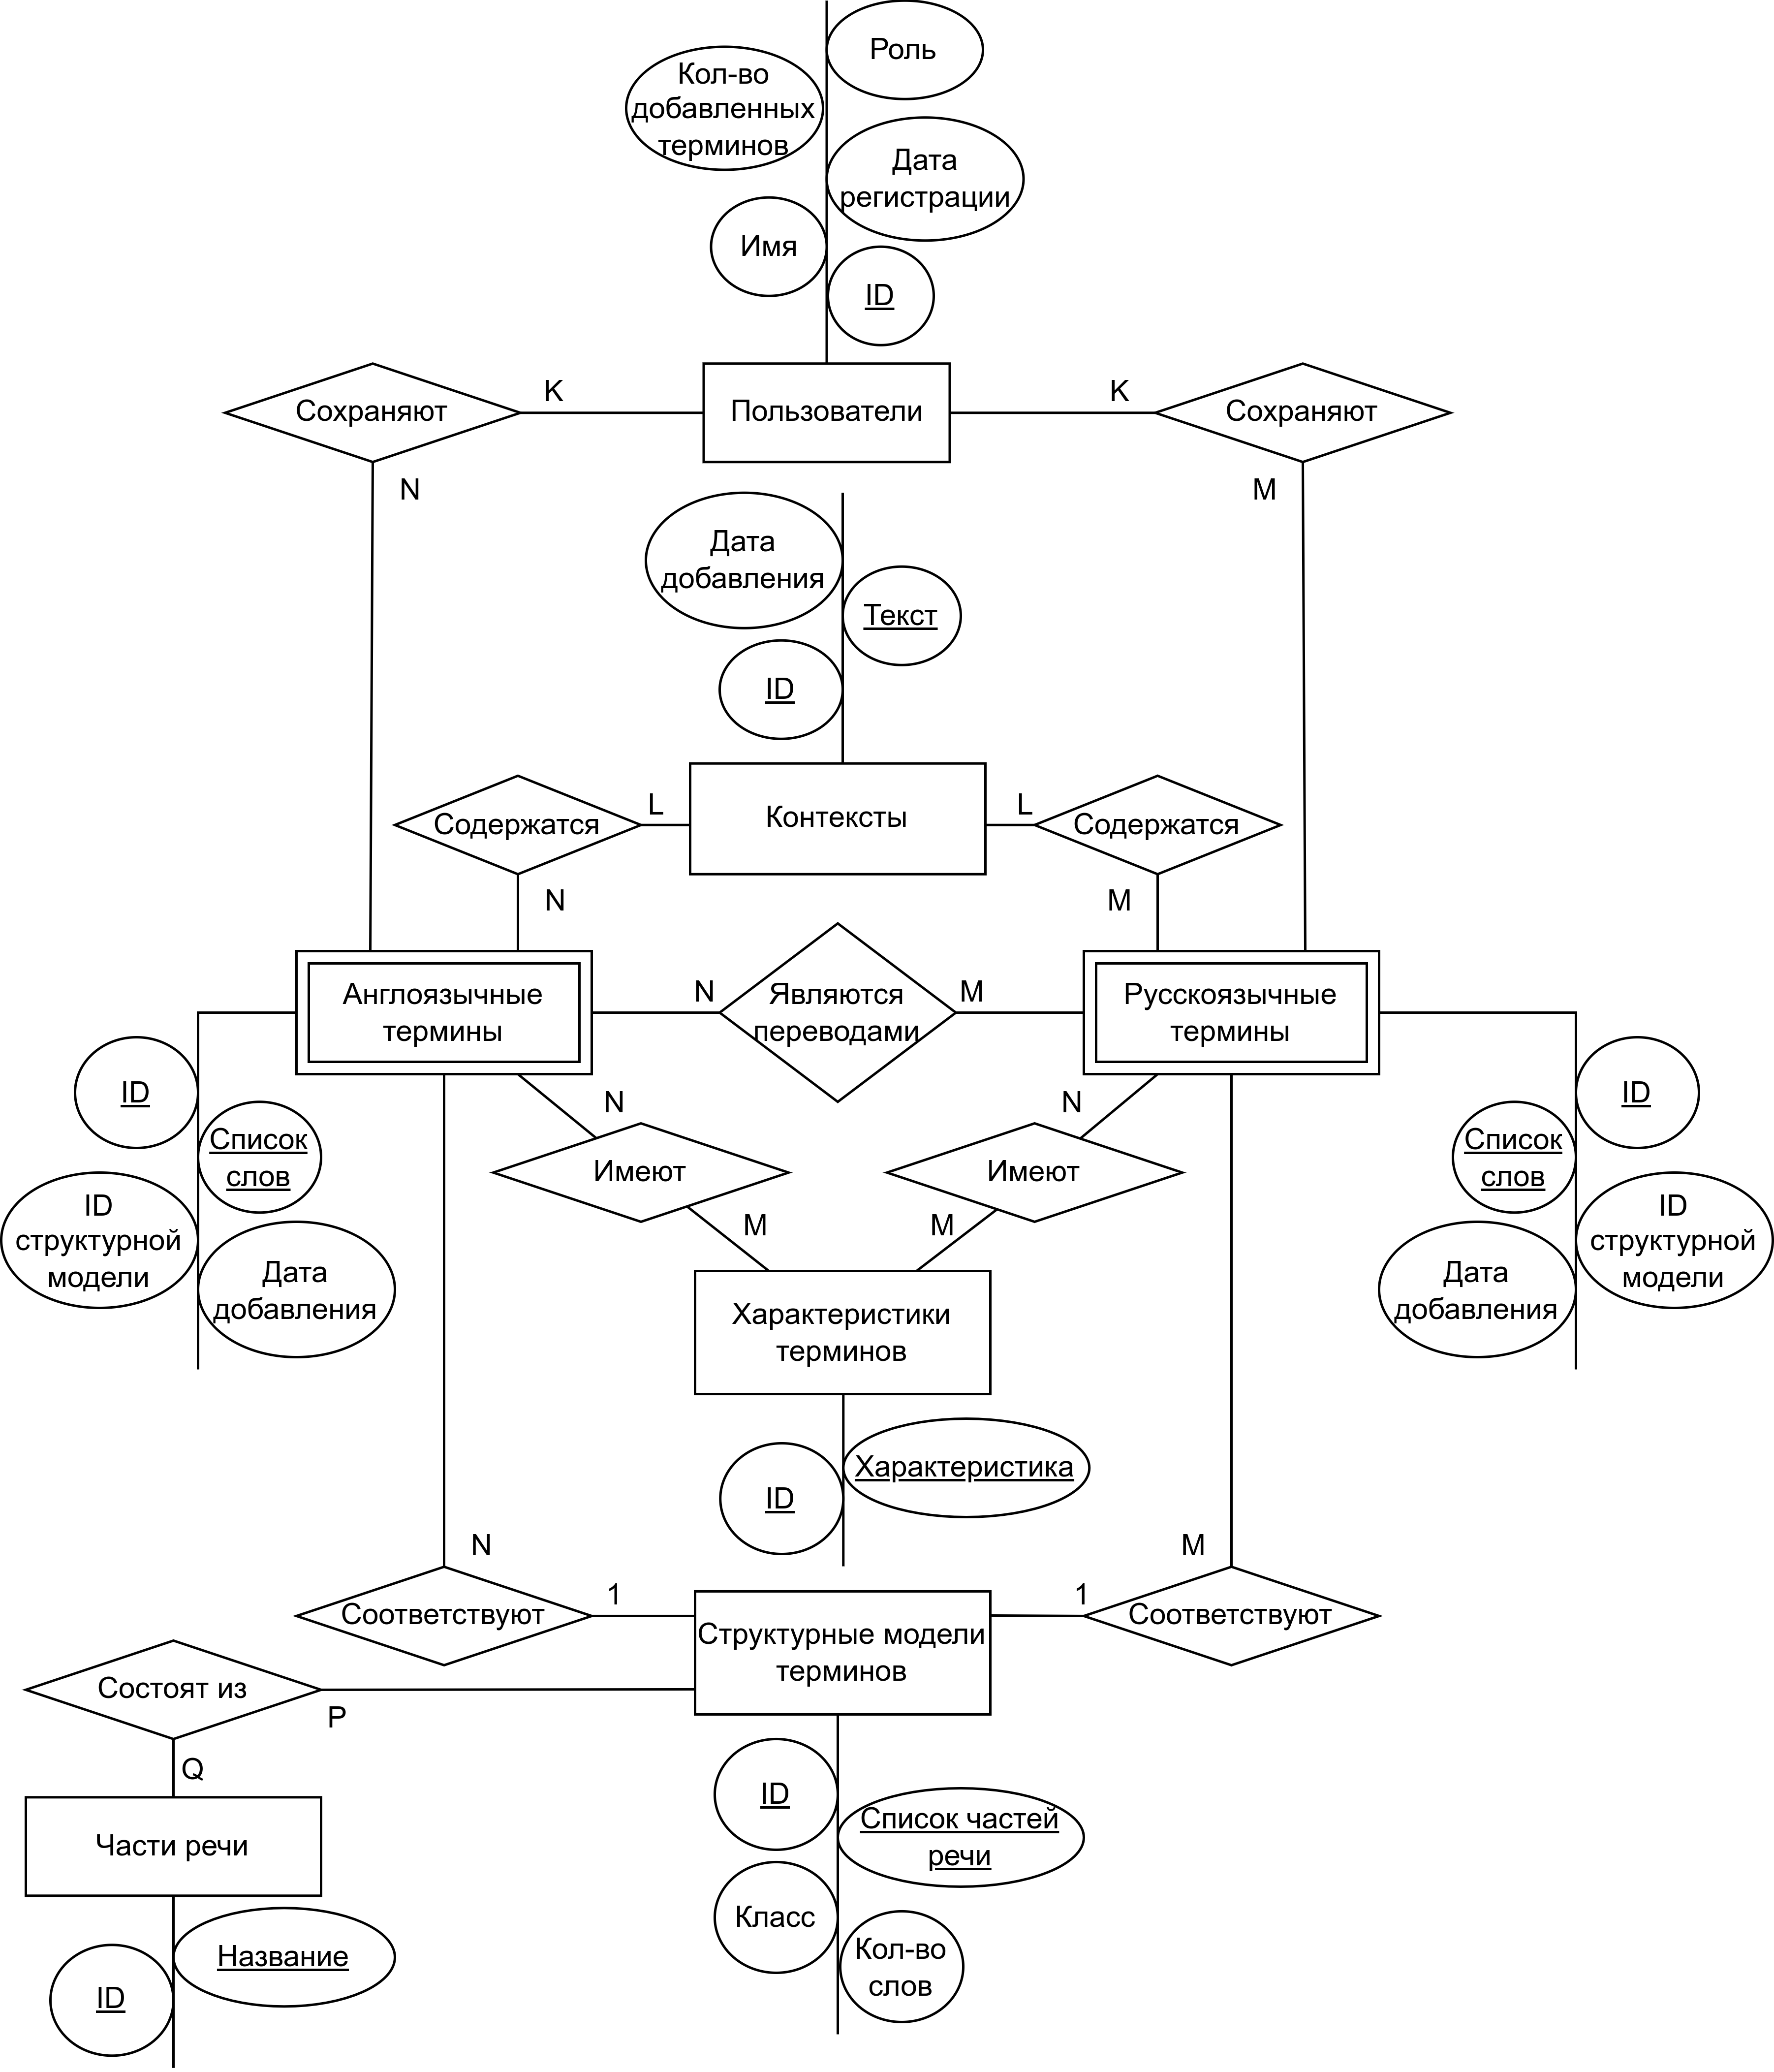
\includegraphics[width=\textwidth ]{img/ER/ER.drawio.png}
	\caption{ER-диаграмма сущностей базы данных}
	\label{fig:er}
\end{figure} 

\clearpage

Стоит отметить, что тексты могут размечаться на нескольких слоях. Это означает, что текст может разбиваться на разные единицы языка и из него можно выделять отдельные слова, термины, синтаксические деревья, семантические падежи и т.д. Соответственно, разрабатываемая база данных должна иметь многослойную структуру: работа с одними и теми же сущностями должна производиться по отдельности для каждого слоя разметки текстов.
% на каждом уровне разметки текста должна производиться работа с сущностями, которые выполняют одинаковые функции, но располагаются на разных слоях разметки текстов.



\subsection{Формализация ролей}

Для работы с системой обязательным этапом является прохождение аутентификации. Пользователь может работать в системе под одной из следующих ролей.

\begin{enumerate}[label*=\arabic*.]
	\item Студент --- пользователь, имеющий возможность обрабатывать тексты, сохранять выделенные термины, а также анализировать и редактировать только те термины, которые он выделил.
	\item Преподаватель --- пользователь, обладающий функционалом, доступным роли <<Студент>>, и имеющий возможность анализировать и редактировать все термины, хранящиеся в базе данных. Таже данной роли доступна функция добавления нового слоя разметки текстов.
	\item Администратор --- пользователь, имеющий возможности, доступные роли <<Преподаватель>>, а также имеющий в распоряжении специальные функции для анализа состояния системы и настройки её работы. Также администратор имеет возможность создавать аккаунты, соответствующие любой из ролей в системе.
	
\end{enumerate}

В ходе использования приложения должна быть предусмотрена возможность смены ролей путём прохождения повторной аутентификации.

Также стоит отметить, что до входа в аккаунт пользователь считается неавторизованным и не имеет доступа к функционалу системы, так как любая работа с терминами должна быть персонализирована.

На рисунке \ref{fig:use-case} представлена диаграмма вариантов использования системы в соответствии с выделенными типами пользователей.

\begin{figure}[h]
	\centering
	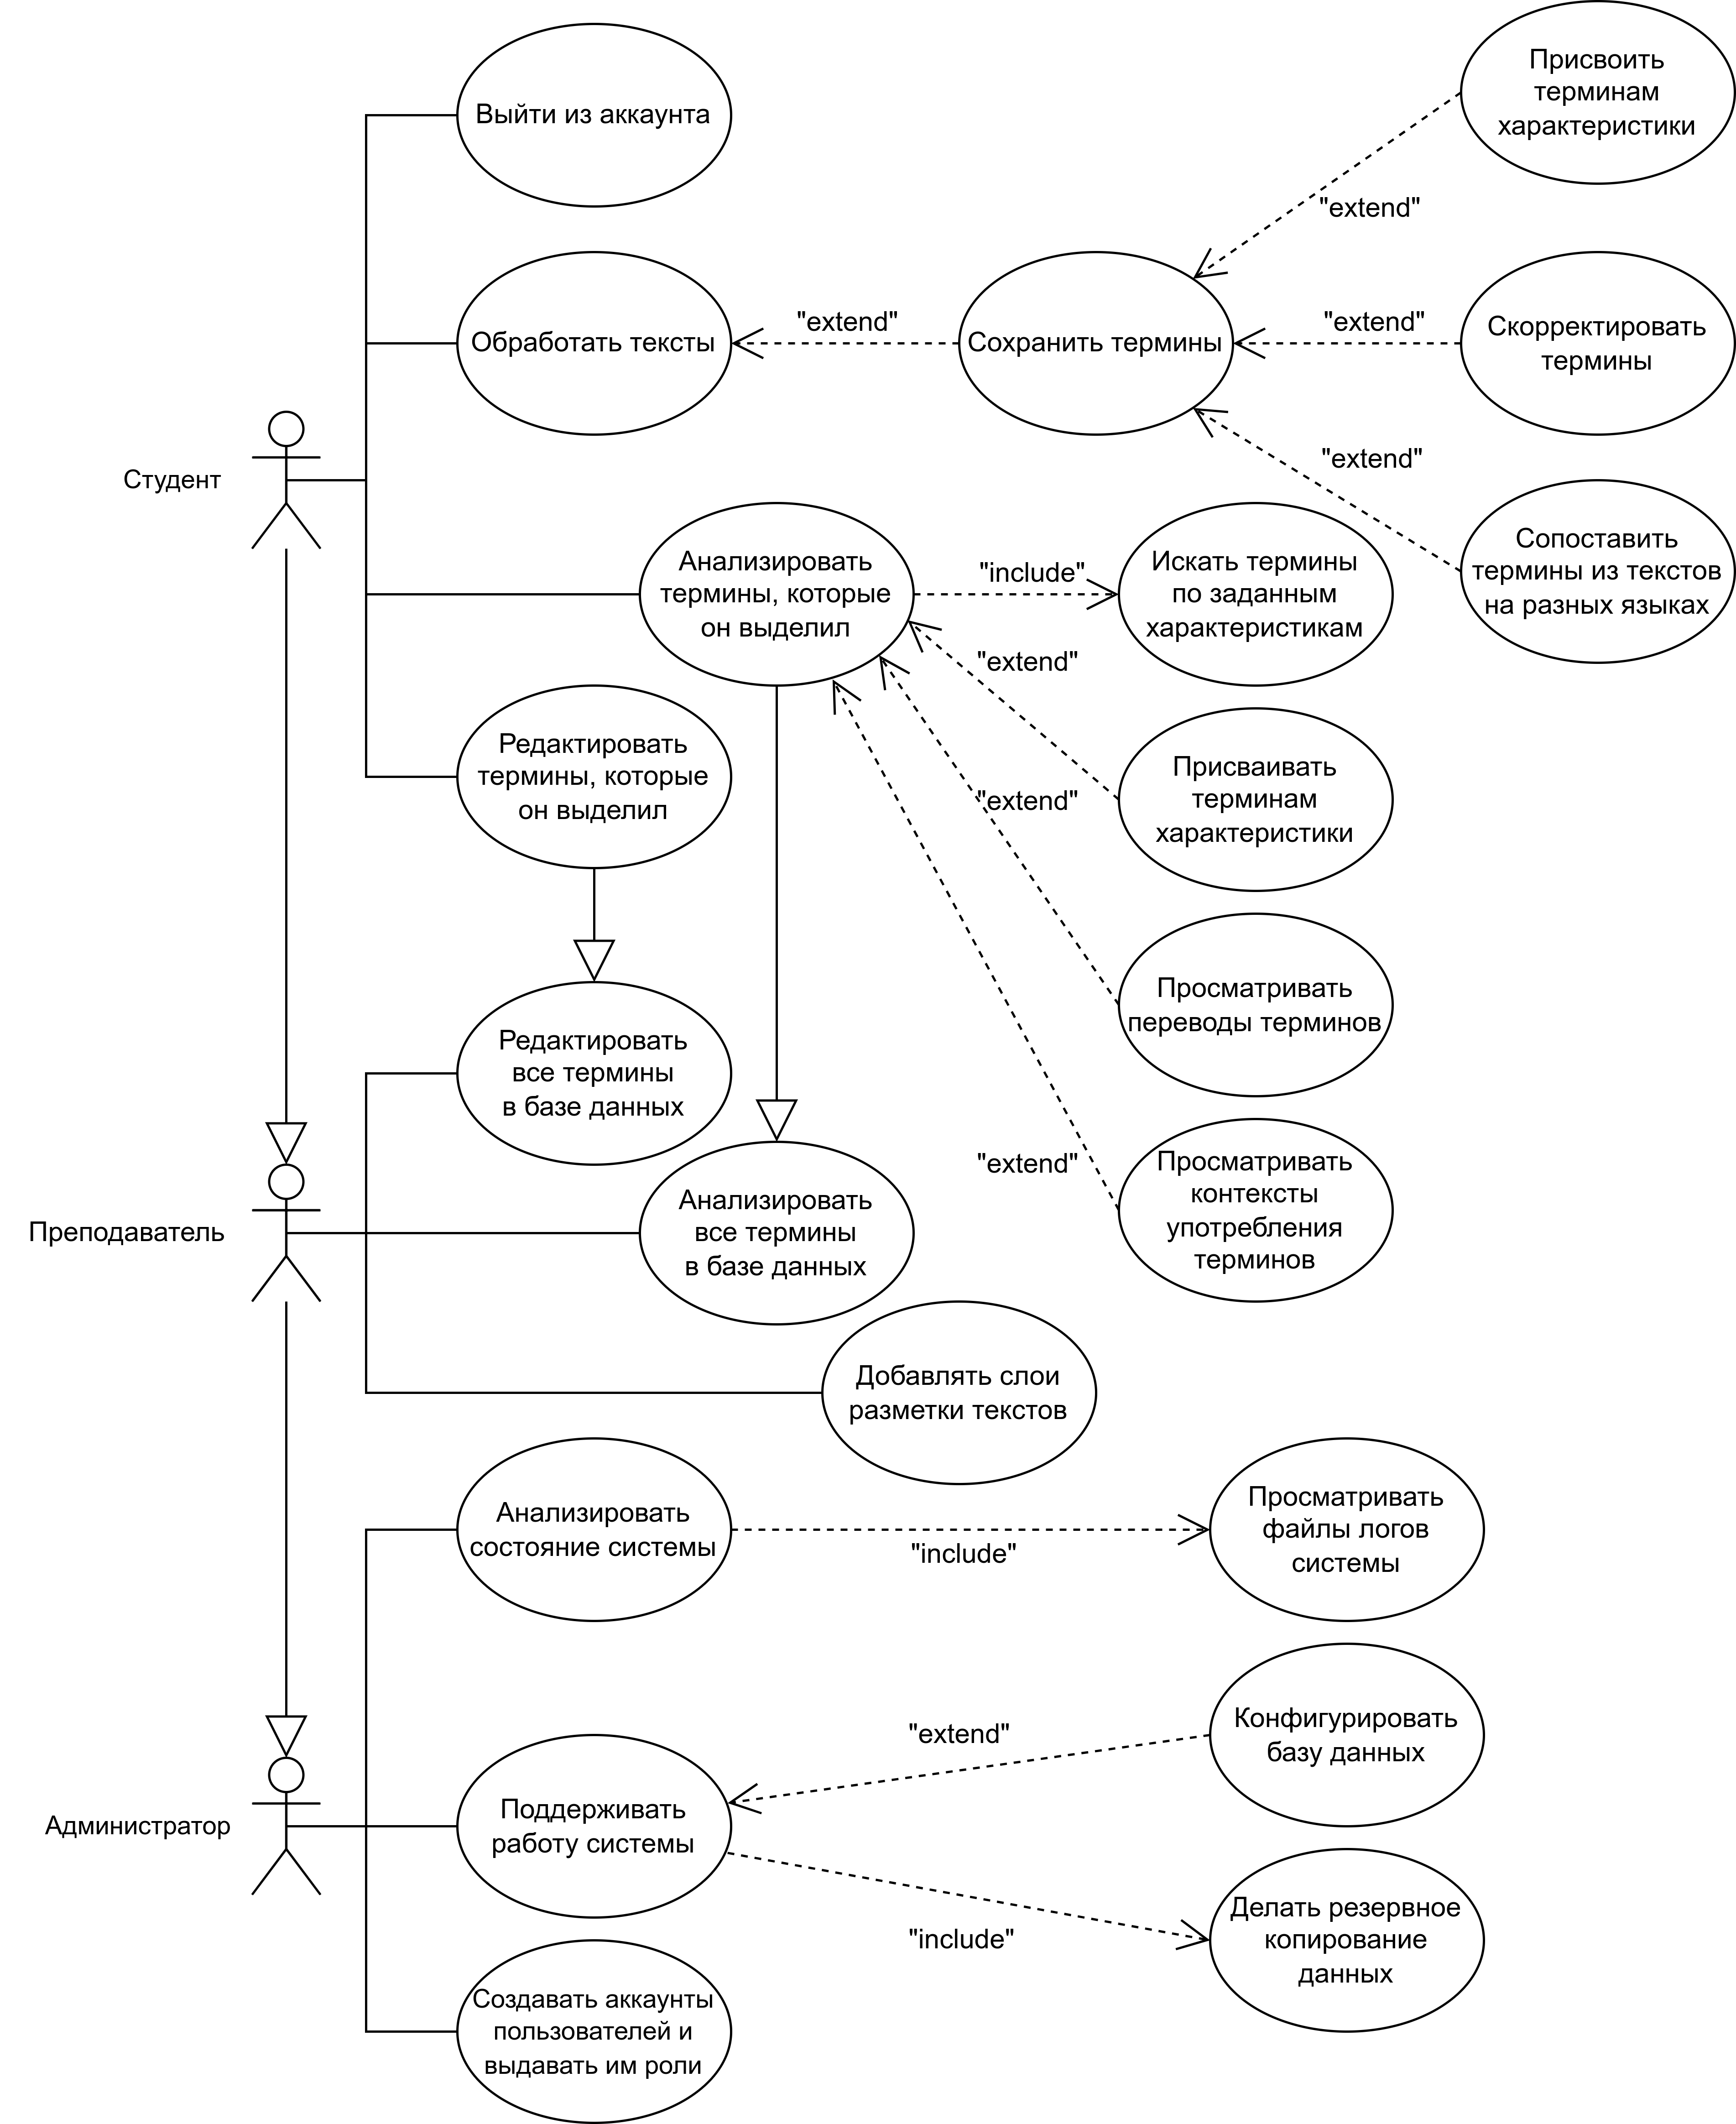
\includegraphics[width=\textwidth ]{img/Use-case/Use-case.drawio.png}
	\caption{Диаграмма вариантов использования}
	\label{fig:use-case}
\end{figure} 

\clearpage



\subsection{Анализ моделей данных}

\subsubsection{Классификация СУБД по модели данных}

По модели данных СУБД можно разделить на следующие типы.

\begin{enumerate}[label*=\arabic*.]
	\item \textbf{Дореляционные}. \newline
	Старые (дореляционные) системы можно разделить на три большие категории: системы с инвертированными списками (inverted list), иерархические (hierarchic) и сетевые (network) \cite{Date_old}. 
	
	% В настоящей книге эти категории подробно не рассматриваются, поскольку, по крайней мере, с точки зрения технологии, их можно считать устаревшими.
		
	\begin{enumerate}[label*=\arabic*.]
		\item \textbf{Инвертированные списки (файлы)}. \newline
		База данных на основе инвертированных списков представляет собой совокупность файлов (таблиц), содержащих записи. Для записей в файле определен некоторый порядок, диктуемый физической организацией данных. Для каждого файла может быть определено произвольное число других упорядочений на основании значений некоторых полей записей (инвертированных списков). Обычно для этого используются индексы. В такой модели данных отсутствуют ограничения целостности как таковые. Все ограничения на возможные экземпляры базы данных задаются теми программами, которые с ней работают. Одно из немногих ограничений, которое может присутствовать --- это ограничение, задаваемое уникальным индексом. 
		
		\item \textbf{Иерархические}. \newline
		Иерархическая модель данных состоит из объектов с указателями от родительских объектов к дочерним, соединяя вместе связанную информацию. Иерархические базы данных могут быть представлены в виде дерева. Их производительность в значительной степени зависит от подхода, выбранного самим пользователем (прикладным программистом и/или администратором базы данных).
		
		\item \textbf{Сетевые}. \newline
		К основным понятиям сетевой модели данных относятся элемент (узел) и связь. Узел --- это совокупность атрибутов данных, описывающих некоторый объект. Сетевые базы данных могут быть представлены в виде графа. В сетевой БД логика процедуры выборки данных зависит от физической организации этих данных. Поэтому эта модель не является полностью независимой от приложения. Другими словами, если необходимо изменить структуру данных, то нужно изменить и приложение.
		
	\end{enumerate}
	
	\item \textbf{Реляционные}. \newline
	Определение реляционной системы требует \cite{Date_old}, чтобы база данных только воспринималась пользователем как набор таблиц. Таблицы в реляционной системе являются логическими, а не физическими структурами. Таблицы представляют собой абстракцию способа физического хранения данных, в которой детали реализации на уровне физической памяти скрыты от пользователя.
	
	Реляционные базы данных основаны на информационном принципе: все информационное наполнение базы данных представлено одним и только одним способом, а именно --- явным заданием значений, помещенных в позиции столбцов в строках таблицы. Этот метод представления --- единственно возможный для реляционных баз данных. В частности, нет никаких указателей, связывающих одну таблицу с другой.
	
	Реляционная модель состоит из следующих компонентов \cite{Date_old}.
	
	\begin{itemize}[label*=---]
		\item  Неограниченный набор скалярных типов (включая, в частности, логический тип).
		\item  Генератор типов отношений и соответствующая интерпретация для сгенерирован ных типов отношений.
		\item  Возможность определения переменных отношения для указанных сгенерированных типов отношений.
		\item  Операция реляционного присваивания для присваивания реляционных значений указанным переменным отношения.
		\item  Неограниченный набор общих реляционных операторов (реляционная алгебра) для получения значений отношений из других значений отношений.
		
	\end{itemize}
	
	% Вполне очевидно, что реляционная модель --- это нечто большее, чем просто "таблицы плюс операции сокращения, проекции и соединения", хотя ее неформально довольно часто характеризуют именно таким образом. 
	
	\item \textbf{Постреляционные}. \newline
	В связи с быстрым ростом количества данных и их усложнением возникла необходимость в поиске новых подходов к хранению и обработке, отличных от реляционных. Таким решением стала NoSQL-технология (Not Only SQL). Постреляционная модель является расширением реляционной модели. Она снимает ограничение неделимости данных, допуская многозначные поля, значения которых не являются атомарными, и набор значений воспринимается как самостоятельная таблица, встроенная в главную \\таблицу \cite{Markin}.
	
	Наиболее популярными типами постреляционных СУБД являются:
	
	\begin{itemize}[label*=---]
		\item ключ-значение (Redis, Tarantool, Oracle NoSQL DB);
		\item колоночные (Vertica, ClickHouse, HBase);
		\item документо-ориентированные (CouchDB, MongoDB);
		\item графовые (InfoGrid, GraphX, Neo4j).
	
	\end{itemize}
	
\end{enumerate}



\subsubsection{Выбор модели данных}

Для долговременного хранения данных будет использоваться реляционная модель по следующим причинам:

\begin{enumerate}[label*=\arabic*)]
	\item данные имеют чётко заданную структуру;
	\item исключается дублирование данных за счёт использования связей между отношениями с помощью внешних ключей;
	\item доступ к данным отделяется от способа их организации на уровне физической памяти;
	
\end{enumerate}

Для кратковременного хранения данных о текущей сессии пользователя (в частности, сохранённых им терминов) будет использоваться нереляционная модель по следующим причинам:

\begin{enumerate}[label*=\arabic*)]
	\item данные могут не иметь общей структуры;
	\item появляется возможность хранения вложенных структур данных;
	\item повышается быстродействие за счёт возможности хранения всех данных в оперативной памяти (In-Memory Database);
	
\end{enumerate}

In-Memory --- набор концепций хранения данных, основанных на их сохранении в оперативной памяти сервера и использовании вторичной памяти для хранения резервных копий. Быстродействие In-Memory баз данных по сравнению с реляционными позволит повысить отзывчивость системы, уменьшив время ожидания пользователя при выполнении сохранения и поиска терминов.



\subsection*{Вывод из аналитической части}

В данном разделе были описан метод извлечения многокомпонентных терминов из научно-технических текстов, на основе которого были сформулированы требования к приложению. Также были описаны сущности базы данных и определены следующие роли пользователей: студент, преподаватель и администратор. Были проанализированы модели данных: для долговременного хранения данных будет использоваться реляционная модель, а для кеширования данных пользовательских сессий --- нереляционная (In-Memory хранилище).



\pagebreak